\documentclass{article}
\usepackage[utf8]{inputenc}
\usepackage{amsmath}
\usepackage{mathtools}
\usepackage[a4paper,left=0.8in,right=0.8in,bottom=1in]{geometry}
\setlength{\parskip}{1em}
\setlength{\parindent}{0.11em}
\usepackage{floatrow}
\usepackage{graphicx}
\title{CS215 Assignment 2}
\author{Aquib Nawaz(190050023),Rajesh Dasari(190050030),\\Paavan Kumar(190050051)}
\date{14 September 2020}

\begin{document}

\maketitle
\section*{Question 1}
    Given , $X_1,X_2,X_3 ,...X_n$ are n identically distributed random variables with cdf $F_X(x)$ and pdf $f_X(x) = F_X'(x)$.\par 
    And $Y_1 = max(X_1,X_2,X_3 ,...X_n)$\\
    We know that the cdf of a variable is $F_X(x) = P(X\leq x)$\\
    Therefore, cdf of $Y_1$  will be ,$F_{Y_1}(y) = P(Y_1 \leq y)$\par 
    $F_{Y_1}(y) = P(max(X_1,X_2,X_3 ,...X_n) \leq y)$\\
    If $max(X_1,X_2,X_3 ,...X_n)$ is less than $y$ ,then each of $X_1,X_2,X_3 ,...X_n$ must be less than y\par
    $F_{Y_1}(y) = P(X_1 \leq y \& X_2 \leq y \& .... \& X_n \leq y)$\\ 
    Since these are independent random variables\par 
    $F_{Y_1}(y) = P(X_1 \leq y)  P(X_2 \leq y)   \dots P(X_n \leq y)$\\
    Each of these is cdf of $X_i$ for i $\epsilon \  1 \dots n$\par 
    $F_{Y_1}(y) = F_X(x)  F_X(x)  \dots F_X(x)$\\
    Therefore,\par 
    $F_{Y_1}(y) = {F_X(x)}^n$\\
    For finding the pdf ,differentiating is sufficient\par
    $f_{Y_1}(y) = n{F_X(x)}^{n-1} f_X(x)$\\
    \hline
    And $Y_1 = min(X_1,X_2,X_3 ,...X_n)$\\
    We know that the cdf of a variable is $F_X(x) = P(X\leq x)$\\
    Therefore, cdf of $Y_1$  will be ,$F_{Y_2}(y) = P(Y_2 \leq y)$\par 
    $F_{Y_2}(y) = P(min(X_1,X_2,X_3 ,...X_n) \leq y)$\par 
    $F_{Y_2}(y) = 1 - P(min(X_1,X_2,X_3 ,...X_n) \geq y)$\\
    If $min(X_1,X_2,X_3 ,...X_n)$ is greater than $y$ ,then each of $X_1,X_2,X_3 ,...X_n$ must be greater than y\par
    $F_{Y_2}(y) = 1 - P(X_1 \geq y \& X_2 \geq y \& .... \& X_n \geq y)$\\ 
    Since these are independent random variables\par 
    $F_{Y_2}(y) = 1 - P(X_1 \geq y)  P(X_2 \geq y)   \dots P(X_n \geq y)$\par 
    $F_{X_i}(x) = P(X_i \leq x) = 1 - P(X_i \geq x)$\\
    Hence ,\par 
    $F_{Y_2}(y) = 1 - (1-F_X(x))(1-F_X(x))  \dots (1-F_X(x)$)\\
    Therefore,\par 
    $F_{Y_2}(y) = 1 -{(1 -F_X(x))}^n$\\
    For finding the pdf ,differentiating is sufficient\par
    $f_{Y_2}(y) = -n{(1-F_X(x))}^{n-1}(-f_X(x))$\par 
    $f_{Y_2}(y) = n{(1-F_X(x))}^{n-1}f_X(x)$
\section*{Question 2}
    Given k mixing probabilities $p_i$'s where $\sum_{i=1}^k p_i = 1$ and $\forall i ,\  0 \leq p_i \leq 1$\\
    Since $X \sim  \sum_{i=1}^k p_i\mathcal{N}(\mu_i,\sigma_i^2)$\par
    We have $\phi_{X}(t) = \sum_{i=1}^k p_{i}\phi_{X_i}(t)$                     (using property of mgf)\par
    $E(X) = \frac{d{\phi_X(t)}}{d{t}}|_{t=0} = \sum_{i=1}^k p_i\frac{d{\phi_{X_i}(t)}}{d{t}}|_{t=0}$\par
    But we know that $\frac{d{\phi_{X_i}(t)}}{d{t}}|_{t=0} = \mu_i$\par
    So, $E(X) = \sum_{i=1}^k p_i\mu_i$\par
    $Var(X) =E(X^2) - E(X)^2$\par
    $E(X^2) = \frac{d^2{\phi_X(t)}}{d{t}^2}|_{t=0}=\sum_{i=1}^k p_i \frac{d^2{\phi_{X_i}(t)}}{d{t}^2}|_{t=0} = \sum_{i=1}^kp_i(\mu_i^2 + \sigma_i^2)$  \hspace{4em}as $E(X_i^2) = \mu_i^2 +\sigma_i^2$\par
    $Var(X) = \sum_{i=1}^kp_i(\mu_i^2 + \sigma_i^2) - (\sum_{i=1}^kp_i\mu_i)^2$\par
    MGF of $X_i$ is $\exp(\mu_it + \frac{\sigma_i^2t^2}{2})$ \par
    MGF of $X$ is $\phi_X(t) = \sum_{i=1}^kp_i\exp(\mu_it + \frac{\sigma_i^2t^2}{2})$ \par
    Given $Z = \sum_{i=1}^kp_iX_i$\par
    Consider $Y_i = p_iX_i$ let $G_i$ and $g_i$ be its CDF and PDF respectively. then,\par
    Also $F_i(x)$ and $f_i(x)$ is CDF and PDF of $X_i$ respectively.\par
    $G_i(y) = P|Y_i \leq y | = P|p_iX_i \leq y| = P|X_i \leq \frac{y}{p_i}| = F_i(\frac{y}{p_i})$\par 
    $g_i(y) = F'_i(\frac{y}{p_i}) =  \frac{1}{p_i}f_i(\frac{y}{p_i}) = \frac{exp(\frac{-(\frac{y}{p_i} - \mu_i)^2}{2\sigma_i^2})}{p_i\sqrt{2\pi}\sigma_i} = \frac{exp(\frac{-(y - pi\mu_i)^2}{2p_i^2\sigma_i^2})}{\sqrt{2\pi}p_i\sigma_i}$\par
    So $Y_i$ is also gaussian random variable with mean $p_i\mu_i$ and variance $p_i^2\sigma_i^2$\par
    Now $Z = \sum_{i=1}^kY_i$\par
    MGF of sum of random variables is product of respective mgf.\par
    $\phi_Z(t) = \prod_{i=1}^k\phi_{Y_i}(t) = \prod_{i=1}^k\exp(p_i\mu_it + \frac{p_i^2\sigma_i^2t^2}{2}) = \exp(\sum_{i=1}^k(p_i\mu_it + \frac{p_i^2\sigma_i^2t^2}{2}))$\par
    $\phi_Z(t)$ can also be written as $\exp(\mu_Zt + \frac{\sigma_Z^2t^2}{2})$\par where $\mu_Z = \sum_{i=1}^kp_i\mu_i$ and $\sigma_Z^2 = \sum_{i=1}^kp_i^2\sigma_i^2$\par so by uniqueness of mgf Z is a gaussian random variable with parameters$(\mu_Z, \sigma_Z^2)$\par
    Now $E(Z) = \mu_Z$\\
    $Var(Z) = \sigma_Z^2$\\
    PDF of Z is $f_Z(x) =  \frac{exp(-\frac{(x-\mu_Z)^2}{2\sigma_Z^2})}{\sqrt{2\pi}{\sigma_Z}}$
\section*{Question 3}
    Consider $\tau > 0$,\\
    By markov's inequality , we have for any non zero random variable X,\\
    $P(X \geq a) \leq \frac{E(X)}{a}$\\
    We have $X - \mu > \tau $ ,where $\tau > 0 $
    Now consider for any $b > 0$,\\
    we have $X- \mu + b > \tau + b$\\
    Since , both the quantities are positive, the solution set of $X- \mu > \tau $ must be a subset of\\
    The solution set S of ${(X-\mu + b)}^2 > {(\tau +b)}^2$\\
    Therefore ,we have $P(X - \mu > \tau ) \leq P({(X-\mu + b)}^2 > {(\tau +b)}^2)$\\
    Applying \textbf{Markov's inequality}\par 
    $P(X - \mu > \tau ) \leq \frac{E({(X-\mu + b)}^2)}{{(\tau +b)}^2}$\par 
    $E({(X-\mu + b)}^2) = E({(X-\mu)}^2) + E(2(X-\mu)b) + E(b^2)$\\
    The term in the middle is anyway zero since $E(X-\mu) = 0 $\par 
    $E({(X-\mu + b)}^2) = \sigma^2 + b^2$\par 
    $P(X - \mu > \tau ) \leq \frac{\sigma^2 + b^2}{{(\tau +b)}^2}$\\
    Let $f(b) = \frac{\sigma^2 + b^2}{{(\tau +b)}^2}$\\
    Since this equation is true for all values of b, so differentiating it w.r.t b,\\
    $f'(b) = \frac{2(\tau b -\sigma^2)}{{\tau +b)}^3}$\\
    Setting $f'(b) = 0 $ yields $b = \frac{\sigma^2}{\tau}$\\
    The equation$f(b)$ yields the value $\frac{\sigma^2}{\sigma^2 +\tau^2}$ at $b =\frac{\sigma^2}{\tau} $\par
    $P(X - \mu > \tau ) \leq \frac{\sigma^2}{\sigma^2 +\tau^2}$\\
    \hline
    Consider $\tau < 0 $\\
    We have $X - \mu > \tau $ ,where $\tau < 0 $
    Now consider for any $b > 0$,\\
    we have $-X+\mu + b < -\tau + b$\\
    Since , both the quantities are positive, the solution set of $-X+\mu > -\tau $ must be a subset of\\
    The solution set S of ${(-X+\mu + b)}^2 < {(-\tau +b)}^2$\\
    Therefore ,we have $P(-X + \mu < -\tau ) \leq P({(-X+\mu + b)}^2 > {(-\tau +b)}^2)$\\
    Applying \textbf{Markov's inequality}\par 
    $P(-X +\mu > -\tau ) \leq \frac{E({(-X+\mu + b)}^2)}{{(-\tau +b)}^2}$\par 
    $E({(-X+\mu + b)}^2) = E({(-X+\mu)}^2) + E(2(-X+\mu)b) + E(b^2)$\\
    The term in the middle is anyway zero since $E(X-\mu) = 0 $\par 
    $E({(-X+\mu + b)}^2) = \sigma^2 + b^2$\par 
    $P(-X +\mu > -\tau ) \leq \frac{\sigma^2 + b^2}{{(-\tau +b)}^2}$\\
    Let $f(b) = \frac{\sigma^2 + b^2}{{(-\tau +b)}^2}$\\
    Since this equation is true for all values of b, so differentiating it w.r.t b,\\
    $f'(b) = \frac{2(-\tau b -\sigma^2)}{{-\tau +b)}^3}$\\
    Setting $f'(b) = 0 $ yields $b = \frac{\sigma^2}{-\tau}$\\
    The equation$f(b)$ yields the value $\frac{\sigma^2}{\sigma^2 +\tau^2}$ at $b =\frac{\sigma^2}{-\tau} $\par
    $P(-X + \mu > -\tau ) \leq \frac{\sigma^2}{\sigma^2 +\tau^2}$\\
    $P(X- \mu > \tau ) = 1- P(\tau < X -\mu) = 1 - P(-X + \mu > -\tau )$\\
    Therefore,\par 
    $P(X- \mu > \tau ) \geq 1 - \frac{\sigma^2}{\sigma^2 +\tau^2}$\\
\section*{Question 4}
    We know that $e^{tX} \geq e^{tx} ,t>0 \iff X \geq x$, since $e^x$  is an increasing function \\
    Applying \textbf{Markov's inequality}\par 
    $P(X \geq x) = P(e^{tX} \geq e^{tx}) \leq \frac{E(e^{tX})}{e^{tx}}$, for $t > 0$\par 
    We also know that $\phi_X(t) = E(e^{tX})$ for $t > 0$\\ 
    Therefore \par 
    $P(X \geq x)  \leq e^{-tx}\phi_X(t)$\\
    We know that $e^{tX} \geq e^{tx} ,t<0 \iff X \leq x$, since $e^x$  is an increasing function \\
    Applying \textbf{Markov's inequality}\par 
    $P(X \leq x) = P(e^{tX} \geq e^{tx}) \leq \frac{E(e^{tX})}{e^{tx}}$, for $t < 0$\par 
    We also know that $\phi_X(t) = E(e^{tX})$ for $t < 0$\\ 
    Therefore \par 
    $P(X \leq x)  \leq e^{-tx}\phi_X(t)$\\
    Applying the above result for the random variable $X = \sum_1^n X_i$,\\
    We get \par 
    $P(X \leq (1+\delta)\mu) \leq e^{-(1+\delta)\mu} \phi_X(t)$\\
    So the problem essentially boils down to calculating an upper bound for MGF of X\par
    $\phi_X(t) = E(e^{tX}) = E(e^{t(X_1+X_2+...+X_n)}) $\par 
    $\phi_X(t) = \prod_1^n E(e^{tX_i})$\\
    Since, the expectation of a bernoulli random variable is $1 +p(e^t -1)$\par 
    $\phi_X(t) = \prod_1^n E(e^{tX_i}) = \prod_1^n (1+p_i(e^t -1))$\\
    Using the equation $1 + x < e^x$\par 
    $\phi_X(t) =\prod_1^n (1+p_i(e^t -1)) \leq \prod_1^n e^{p_i(e^t -1)}$\par 
    $\phi_X(t) \leq e^{\sum_1^n p_i(e^t - 1)} = e^{\mu(e^t - 1)}$\par 
    $P(X \leq (1+\delta)\mu) \leq e^{-(1+\delta)\mu} \phi_X(t)$\par
    $P(X \leq (1+\delta)\mu) \leq \frac{e^{\mu(e^t - 1)}}{e^{(1+\delta)\mu}}$
\section*{Question 5}
\subsection*{a)}
    The code for this part is attached with the name \textbf{q5a.m}\par 
    The code on execution produces 10 images with names as N.png where n belongs to [5,10,20,100,200,500,1000,5000,10000]\par 
    Here are the images attached for N = 100,1000 and 10000, using nsamp = 2000\par 
    \begin{figure}[H]
    \begin{floatrow}
    \ffigbox{\caption {Plot for N = 100}}
    {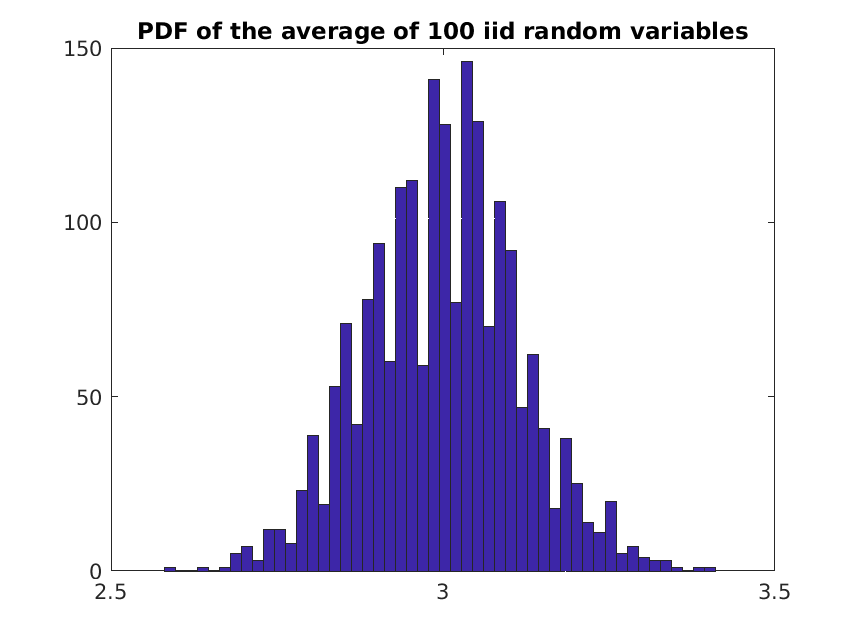
\includegraphics[width =9cm, height=7cm]{100.png}}
    \ffigbox{\caption {Plot for N = 1000}}
    {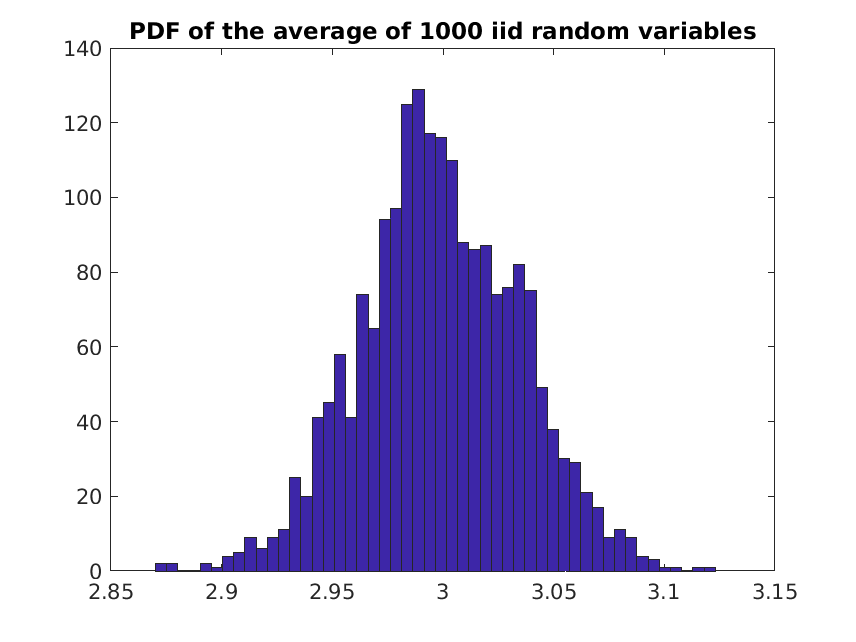
\includegraphics[width =9cm, height=7cm]{1000.png}}
    \end{floatrow}
    \ffigbox{\caption {Plot for N = 10000}}
    {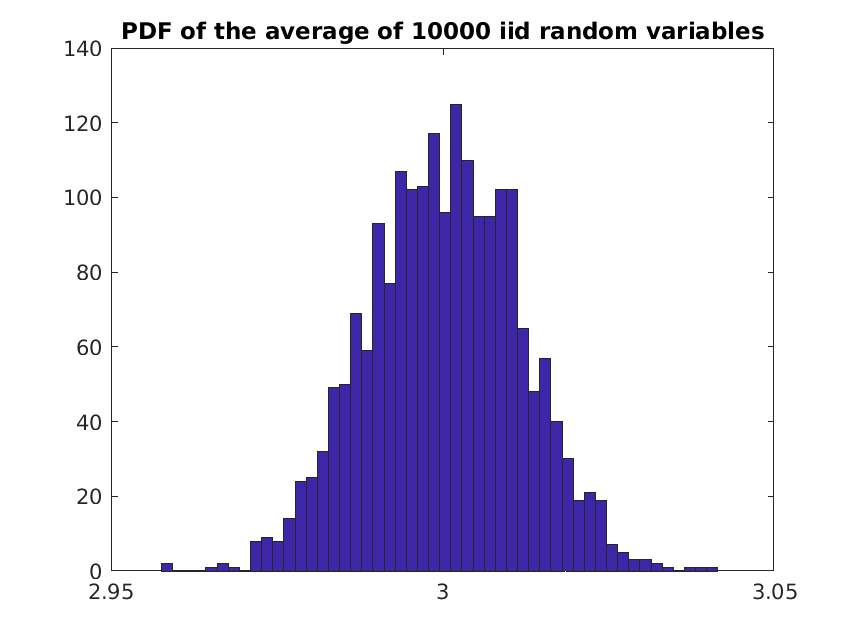
\includegraphics[width =12cm, height=9cm]{10000.png}}
    \end{figure}
\subsection*{b),c)} 
    The code for this part is attached with the name \textbf{q5bc.m}\par
    The code on execution produces 11 images with the first 10 images for part \textbf{b)} and the last image for part \textbf{c)}
    Here are the images attached for N = 100,1000 and 10000.\par 
    \begin{figure}[H]
    \begin{floatrow}
    \ffigbox{\caption {Plot for N = 100}}
    {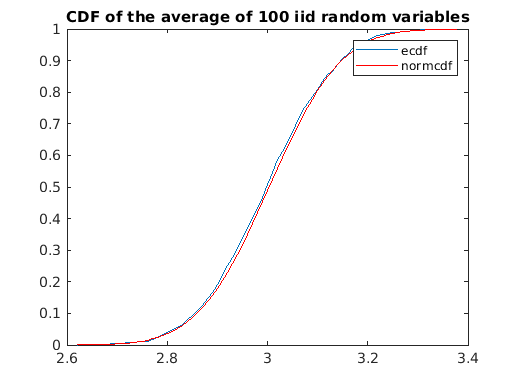
\includegraphics[width =9cm, height=8cm]{1.png}}
    \ffigbox{\caption {Plot for N = 1000}}
    {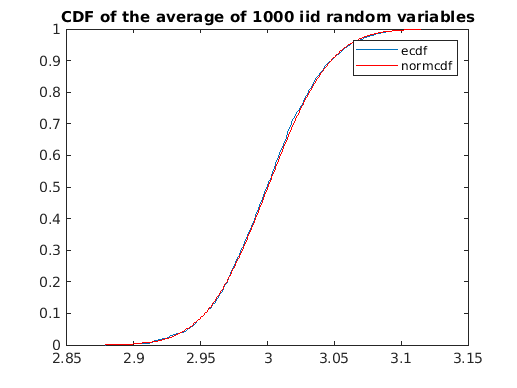
\includegraphics[width =9cm, height=8cm]{2.png}}
    \end{floatrow}
    \ffigbox{\caption {Plot for N = 10000}}
    {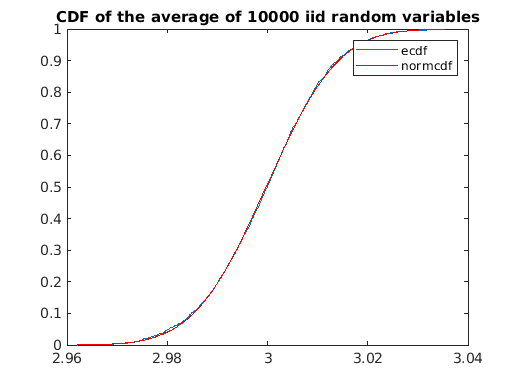
\includegraphics[width =13cm, height=10cm]{3.png}}
    \end{figure}
    \begin{figure}[H]
    \ffigbox{\caption {Plot for MAD versus N}}
    {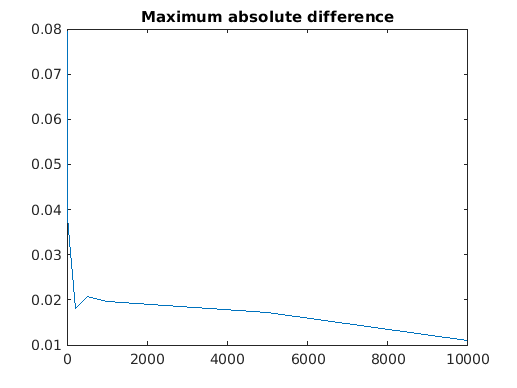
\includegraphics[width =13cm, height=10cm]{4.png}}
    \end{figure}
\section*{Question 6}
    \textbf{Correlation Coefficient}
    \begin{figure}[H]
    \begin{floatrow}
    \ffigbox{\caption {Plot of $\rho$ versus $t_i$ for I2}}
    {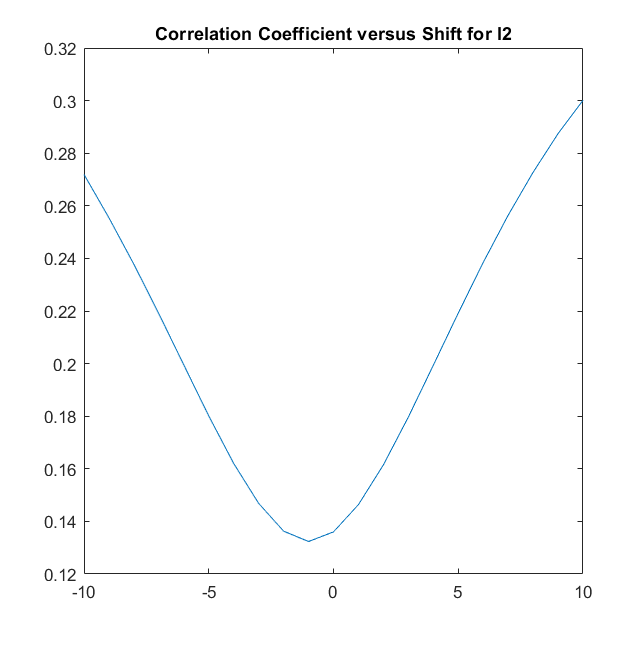
\includegraphics[width =9cm, height=9cm]{fig1.png}}
    \ffigbox{\caption {Plot of $\rho$ versus $t_i$ for I2 =255-I1}}
    {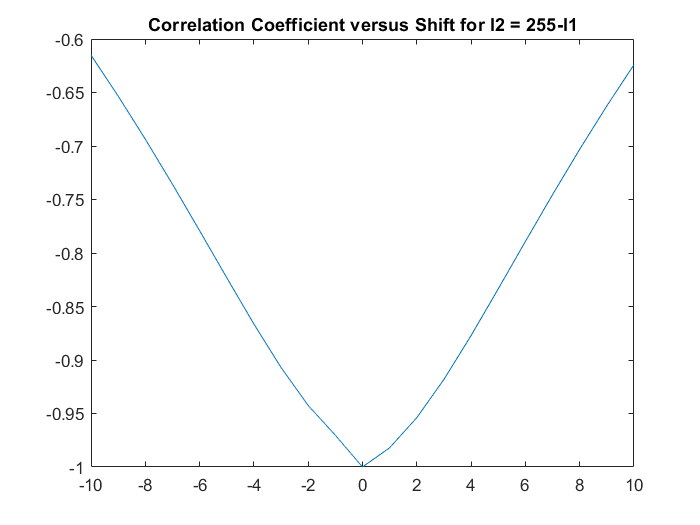
\includegraphics[width =9cm, height=9cm]{fig2.png}}
    \end{floatrow}
    \end{figure}\par 
    For \textbf{I2}\\
    The correlation coefficient is minimum at $t_i = -1$ and it is decreasing as $t_i$ goes from -10 to -1 since the distance b/w aligned pixels is going to decrease and then starts increasing from 0 to 10 because the distance between aligned pixels is increasing resulting in positive corelation-coefficient as  the two images are closely related to each other\par 
    For \textbf{I2 = 255 -I1}\\
    The magnitude of correlation coefficient is maximum at $t_i = 0$ and it is increasing as $t_i$ goes from -10 to -1 since the distance b/w aligned pixels is going to decrease and then starts decreasing from 0 to 10 because the distance between aligned pixels is increasing resulting in negative  corelation-coefficient as  the two images are opposites of each other, the negative corelation coefficient means that the images are negatively corelated and hence -$\rho$ looks same like that plotted for $I2$\par 
    \begin{figure}[H]
    \begin{floatrow}
    \ffigbox{\caption {Plot of $QMI$ versus $t_i$ for I2}}
    {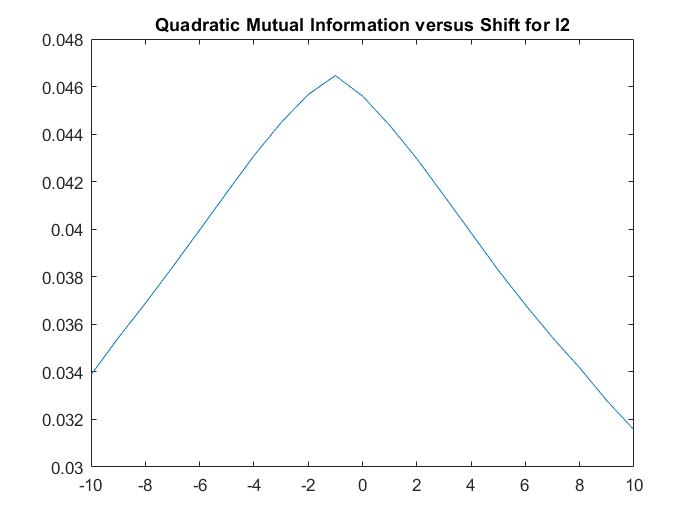
\includegraphics[width =9cm, height=9cm]{f1.png}}
    \ffigbox{\caption {Plot of $QMI$ versus $t_i$ for I2 =255-I1}}
    {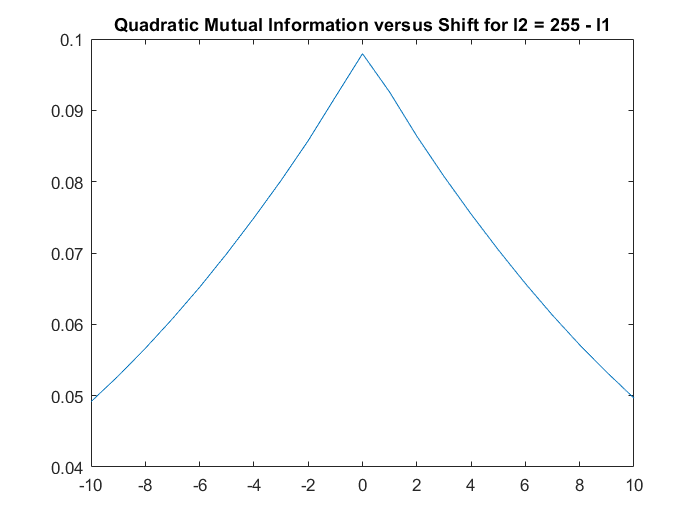
\includegraphics[width =9cm, height=9cm]{f2.png}}
    \end{floatrow}
    \end{figure}\par
    For \textbf{I2}\\
    The Quadratic mutual information that is stored in QMI will be largest at $t_i  = -1$, which also agrees with the fact that the correlation coefficient is minimum at $t_i = -1$ and the values of QMI decrease on either side of $t_i = -1$.This may be the charectersitic of the given images I1,I2. And also the QMI gradually falls to zero as the corelation coefficient increases\par 
    For \textbf{I2 = 255 -I1}\\
    The Quadratic Mutual information stored in QMI will be largest when the two are least co-related since one of the image is inverse of the other image and this is due to the fact that each element is squared in calculation of QMI.The QMI hence decreases on either side of $t_i = 0$ since at $t_i = 0$,the images are negatives of each other,and one can observe that QMI falls to zero as the magnitude of corelation coefficient decreases or rather the corelation coefficient increases (since,it is negative)\par 
    From these graphs one can conclude that QMI is invesely dependent on corelation-coefficient\par 
    The code for this part is attached with the name \textbf{q6.m}
\section*{Question 7}
    The moment generating function of Multinomial random variable is given by,\par
    $\phi_X(\vec t \ ) = E(e^{\vec t \Vec{X}}) = {(\sum_1^n p_i e^{t_i})}^n$ where $p_i, n$ are parameters of multinomial random variable\\
    Now , we have \par 
    $\frac{\partial \phi_X(\vec t \ )}{\partial t_i} = E (\frac{\partial e^{\vec t \Vec{X}} }{\partial t_i})  = E(X_i e^{\vec t \Vec{X}})$\par 
    And for $i,j$\par 
    $\frac{\partial }{\partial t_j}({\frac{\partial \phi_X(\vec t \ )}{\partial t_i}}) = E(\frac{\partial }{\partial t_j}(X_i e^{\vec t \Vec{X}})) = E(X_iX_je^{\vec t \Vec{X}})$\par 
    But also,\par 
    $\frac{\partial \phi_X(\vec t \ )}{\partial t_i} = \frac{\partial }{\partial t_i}({(\sum_1^n p_i e^{t_i})}^n) = n {(\sum_1^n p_i e^{t_i})}^{n-1} {(\sum_1^n \frac{\partial }{\partial t_i}(p_i e^{t_i}))} = np_ie^{t_i} {(\sum_1^n p_i e^{t_i})}^{n-1} $\par 
    For $i = j$\par 
    $\frac{\partial }{\partial t_i}({\frac{\partial \phi_X(\vec t \ )}{\partial t_i}}) = \frac{\partial }{\partial t_i}(np_ie^{t_i} {(\sum_1^n p_i e^{t_i})}^{n-1}) = n(n-1)p_ie^{t_i} {(\sum_1^n p_i e^{t_i})}^{n-2}{(\sum_1^n \frac{\partial }{\partial t_j}(p_i e^{t_i}))} + np_ie^{t_i} {(\sum_1^n p_i e^{t_i})}^{n-1} $\par  
    $({\frac{\partial^2 \phi_X(\vec t \ )}{\partial t_i^2}})= n(n-1)p_i^2e^{2t_i} {(\sum_1^n p_i e^{t_i})}^{n-2} + np_ie^{t_i} {(\sum_1^n p_i e^{t_i})}^{n-1} $\par
    And for $i \neq j$\par
    $\frac{\partial }{\partial t_j}({\frac{\partial \phi_X(\vec t \ )}{\partial t_i}}) = \frac{\partial }{\partial t_j}(np_ie^{t_i} {(\sum_1^n p_i e^{t_i})}^{n-1}) = n(n-1)p_ie^{t_i} {(\sum_1^n p_i e^{t_i})}^{n-2}{(\sum_1^n \frac{\partial }{\partial t_j}(p_i e^{t_i}))} = n(n-1)p_ip_je^{t_i}e^{t_j} {(\sum_1^n p_i e^{t_i})}^{n-2}$\par 
    We know that Variance($X_i$) $= E(X_i^2) - E(X_i)^2$\par 
    $E(X_i^2) = n(n-1)p_i^2 +np_i$ letting $\vec t = \vec 0$\par 
    $a_{ii} = n(n-1)p_i^2 +np_i - n^2p_i^2$\par 
    $a_{ii} = np_i(1-p_i)$\par 
    We know that Covariance($X_i,X_j$) = $E(X_iX_j) - E(X_i)E(X_j)$\par 
    $E(X_iX_j) = n(n-1)p_ip_j $ for $i \neq j$ put $\vec t  = \vec  0$ \par 
    $E(X_i)E(X_j) = (n p_i)( n p_j) = n^2 p_ip_j$\par 
    $a_{ij} = a_{ji} = n(n-1)p_ip_j - n^2 p_ip_j = -np_ip_j$ for $i \neq j$\par 
    $a_{ij} = -np_ip_j $ for $i \neq j$ \par 
\end{document}